%% ===========================================================================
%%  FPV 2026 -- Model-Based Rotor-Rate Control of a 2.5-inch Quadrotor
%%  IEEEtran conference format.  Compile on Overleaf: see README.md
%%
%%  Sections marked with \stub{} are deliberately incomplete -- the data does
%%  not exist yet.  Search for "\stub" to find every one of them.
%% ===========================================================================

\documentclass[conference]{IEEEtran}

\IEEEoverridecommandlockouts

\usepackage{cite}
\usepackage{amsmath,amssymb,amsfonts}
\usepackage{graphicx}
\usepackage{textcomp}
\usepackage{url}
\usepackage{xcolor}
\usepackage{booktabs}
\usepackage{balance}

\graphicspath{{figures/}}

\def\BibTeX{{\rm B\kern-.05em{\sc i\kern-.025em b}\kern-.08em
    T\kern-.1667em\lower.7ex\hbox{E}\kern-.125emX}}

%% ---- marker for the sections that still need work -------------------------
\newcommand{\stub}[1]{%
  \par\smallskip\noindent
  \fcolorbox{black!45}{black!6}{%
    \parbox{0.94\columnwidth}{\footnotesize\textsf{\textbf{[SECTION INCOMPLETE]}}\\[2pt]#1}%
  }\par\smallskip}

%% shorthand
\newcommand{\kF}{k_{F}}
\newcommand{\kM}{k_{M}}
\newcommand{\dps}{\ensuremath{^{\circ}\!/\mathrm{s}}}

\begin{document}

\title{Model-Based Rotor-Rate Control of a 2.5-Inch Quadrotor\\
with Bidirectional DShot Speed Feedback}

\author{\IEEEauthorblockN{D. Benedetti}
\IEEEauthorblockA{\textit{FPV 2026 Project}\\
% TODO: replace with your department, course number and term.
\textit{California Polytechnic State University}\\
San Luis Obispo, CA, USA \\
dmbenedetti777@gmail.com}
}

\maketitle

\begin{abstract}
This paper describes the design, implementation and initial flight testing of
a model-based flight controller for a 163~mm quadrotor built around a single
ESP32 microcontroller. The controller differs from conventional small-airframe
firmware in two respects. First, every sign convention---body axes, sensor
mounting transforms and rotor spin directions---is derived from one declared
right-handed frame in a single header file, after an earlier build was found
to contain a yaw-rate variable whose stored polarity contradicted its name and
which was consumed inconsistently by four separate subsystems. Second, control
is expressed in physical units throughout: the outer loops command
accelerations, the rate loops command angular accelerations that become
torques through the airframe inertia tensor, a control allocator inverts the
rotor geometry to produce four angular-velocity setpoints, and only the
innermost loop---closed on mechanical rotor speed recovered from bidirectional
DShot telemetry---converts to actuator counts. State estimation uses a
nine-error-state Kalman filter fusing an inverted six-axis IMU, a downward
time-of-flight rangefinder, an optical-flow sensor and a magnetometer.
A saturation policy that prioritises roll and pitch over thrust and thrust
over yaw is shown to be necessary on this airframe, where yaw authority is
0.042~N$\cdot$m against 0.34~N$\cdot$m in roll and pitch. Flight tests
demonstrate hands-off hover with $1.1^{\circ}$ standard deviation in roll and
$1.2^{\circ}$ in pitch, 22~mm standard deviation in altitude, and no allocator
saturation across 917 logged control frames. A persistent 55~mm altitude
offset is traced quantitatively to a 4.8\% error in the modelled thrust
coefficient combined with the deliberate absence of an integral term in the
vertical cascade.
\end{abstract}

\begin{IEEEkeywords}
quadrotor, control allocation, error-state Kalman filter, optical flow,
rotor speed control, DShot, embedded control
\end{IEEEkeywords}

%% ===========================================================================
\section{Introduction}

Small multirotor flight controllers conventionally map three independent
attitude PID outputs directly onto motor commands through a hand-written mixer
matrix~\cite{bouabdallah2007,mahony2012}. The approach is compact and works
well when the mixer signs are correct, but it offers no way to detect that
they are not. Each PID gain is expressed in actuator counts per unit of error,
so it absorbs the motor curve, the battery state and the propeller constant
along with the airframe dynamics, and none of those quantities can be reasoned
about separately.

This work re-implements the controller for a 163~mm quadrotor around two
principles.

\textbf{Conventions are declared once.} A single header defines the body frame
as $+X$ right, $+Y$ forward, $+Z$ up, declares every rotation right-handed,
and derives each sensor mounting transform from measurement. The motivation
was concrete: in the preceding build, a variable holding a measured yaw rate
was named as clockwise-positive but stored a counter-clockwise value. Three
consumers assumed the name and one assumed the value. The result was a yaw
mixer closing positive feedback, a magnetic heading fed to the estimator with
inverted sign, and body-to-navigation rotations written as each other's
transpose---invisible at zero heading, fully cross-coupled at $90^{\circ}$.
Roll and pitch were unaffected, which is precisely why the fault survived
several flight campaigns.

\textbf{Control is expressed in physical units.} The signal path runs
position~$\rightarrow$~velocity~$\rightarrow$~acceleration~$\rightarrow$~tilt,
then tilt~$\rightarrow$~body~rate~$\rightarrow$~angular~acceleration~$\rightarrow$
torque, then (thrust, torque)~$\rightarrow$~per-rotor angular velocity, and
finally angular velocity~$\rightarrow$~actuator counts through a loop closed on
measured rotor speed. Every gain is therefore a physical quantity, and the
mixer is computed from rotor positions and spin directions rather than written
down, so a sign error would have to be a geometry error. This places the
design in the control-allocation framework surveyed by Johansen and
Fossen~\cite{johansen2013}, with the airframe model of Bangura and
Mahony~\cite{bangura2012} supplying the effectiveness matrix.

Section~\ref{sec:arch} describes the hardware and the radio link.
Section~\ref{sec:model} sets out the frame conventions, documents the fault
that motivated them, and develops the motion model and control-effectiveness
matrix. Sections~\ref{sec:sensors} and~\ref{sec:estimator} cover the sensor
stack and the state estimator. Sections~\ref{sec:control}--\ref{sec:rotor}
describe the control cascade, the allocator and the rotor speed loop.
Section~\ref{sec:impl} covers the embedded implementation,
Section~\ref{sec:results} the flight test results, and
Section~\ref{sec:limits} the defects that remain.

%% ===========================================================================
\section{System Architecture}
\label{sec:arch}

\begin{figure*}[!t]
\centering
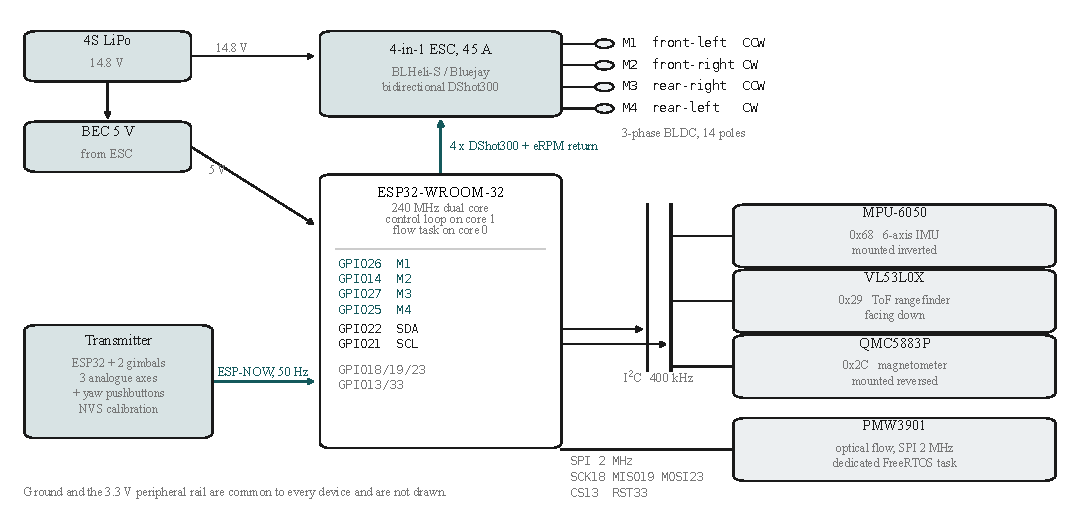
\includegraphics[width=\textwidth]{fig_wiring.pdf}
\caption{System interconnect. A single ESP32 runs the entire control stack.
Three sensors share one \mbox{I\textsuperscript{2}C} bus; the optical-flow
sensor is on a dedicated SPI bus serviced by its own FreeRTOS task pinned to
the opposite core, because its burst read is long enough to disturb the
control cadence if performed inline. The four DShot lines are bidirectional:
the same wire carries the throttle command outbound and the electrical-period
telemetry frame inbound, which is what makes the rotor speed loop of
Section~\ref{sec:rotor} possible without additional wiring.}
\label{fig:wiring}
\end{figure*}

The aircraft is a 163~mm X-configuration quadrotor with 2.5-inch propellers,
a four-in-one 45~A electronic speed controller running Bluejay
firmware~\cite{bluejay}, and a single ESP32-WROOM-32~\cite{esp32} as the only
flight computer. There is no dedicated flight-controller board; the ESP32
performs sensing, estimation, control, allocation, actuator drive and
telemetry. Fig.~\ref{fig:wiring} shows the interconnect.

\subsection{Radio link and transmitter}

The radio link is ESP-NOW between two ESP32 modules. The transmitter sends a
fixed-layout packet every 20~ms (50~Hz) carrying a magic word, a sequence
number, four axis values and two boolean switches. Loss of the link for more
than 300~ms zeroes all stick inputs and releases the arm.

The transmitter reads throttle, roll and pitch from three ADC channels on two
gimbals. Yaw is taken by default from the two gimbal pushbuttons rather than a
potentiometer, commanding a fixed $\pm45$~\dps\ through a 150~ms slew. That
choice suits a heading-hold controller: releasing a button returns an exact
zero, so the receiver's heading capture sees a clean stick-inactive edge
instead of potentiometer noise hovering near the deadband. An analogue fourth
axis is supported but not fitted.

Stick calibration is stored in the ESP32's non-volatile storage rather than
recompiled into the source, so it survives power cycles and boot is immediate.

Two properties of this interface are worth stating because they are easy to
get wrong. Throttle is a \emph{centred} axis---centre commands hold, up
climbs, down descends---so arming requires the stick near mid-travel, not at
the bottom of its throw. And the transmitter deliberately transmits
throttle~$=-1.0$ when switched off or killed, which the receiver treats as a
sentinel rather than a fault.

\stub{Transmitter ergonomics and the pilot interface are described only
functionally here. A photograph of the transmitter and the airframe, and a
bench photograph showing sensor placement relative to the power leads, would
support Section~\ref{sec:limits}, where magnetometer proximity to the power
wiring is identified as an unresolved defect.}

\subsection{Sensing and actuation}

Four sensors feed the estimator. An MPU-6050~\cite{mpu6050} provides angular
rate and specific force at the control rate. A VL53L0X~\cite{vl53l0x}
time-of-flight rangefinder measures height above the floor. A
PMW3901~\cite{pmw3901} optical-flow sensor measures translational rate over
the floor. A QMC5883P~\cite{qmc5883p} magnetometer provides an absolute
heading reference. The IMU is installed inverted and the magnetometer is
installed reversed; both are handled by fixed transforms rather than by
per-axis sign constants scattered through the code.

%% ===========================================================================
\section{Frames, Airframe and Motion Model}
\label{sec:model}

\begin{figure*}[!t]
\centering
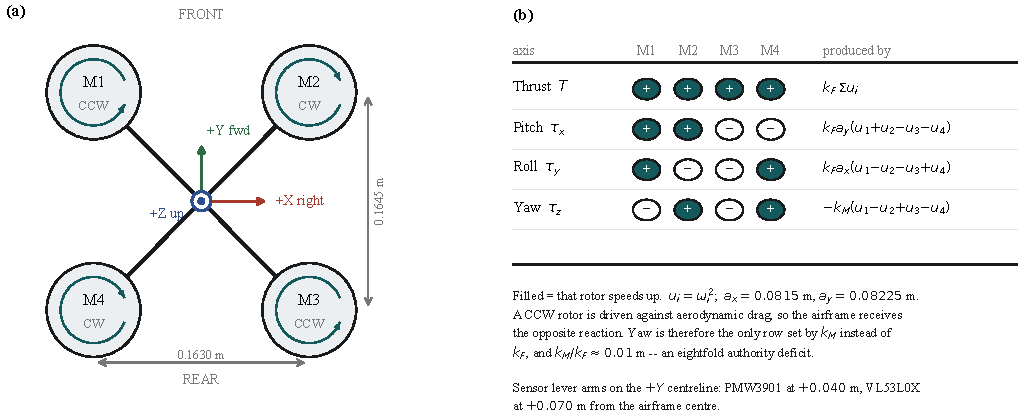
\includegraphics[width=\textwidth]{fig_body.pdf}
\caption{(a) Body frame and rotor layout, viewed from above. Rotations are
right-handed about the drawn axes, so roll is a rotation about $+Y$ and pitch
about $+X$; a clockwise turn seen from above is a \emph{negative} $\omega_z$.
(b) Control effectiveness. Because the forward map is linear in
$u_i=\omega_i^2$, the inverse used by the allocator is closed form. The yaw
row is the only one whose magnitude is set by $\kM$ rather than $\kF$, and
that single fact drives the saturation policy of
Section~\ref{sec:alloc}.}
\label{fig:body}
\end{figure*}

\subsection{Frames, and a case study in why they are declared once}

The body frame is $+X$ right, $+Y$ forward, $+Z$ up, with every rotation
right-handed. Two consequences of that definition are stated explicitly
because they are the ones that trip people:
\emph{roll is a rotation about $+Y$ and pitch about $+X$}, and \emph{a
clockwise turn seen from above is a negative $\omega_z$}. There is no
clockwise-positive quantity anywhere in the build.

The navigation frame is captured at each estimator reset, with $+X_n$ and
$+Y_n$ aligned to the body axes at that instant. Body-to-navigation is the
standard right-handed rotation, and navigation-to-body is its transpose---the
two are true inverses, which the previous build's pair were not.

Table~\ref{tab:faults} records what the earlier convention fault actually did,
because it motivates the whole structure of this section. A single variable
held a counter-clockwise-positive rate under a clockwise-positive name. Four
consumers disagreed about which was true, and each failed differently. Notably
none of the four is a tuning problem, and no gain change could have addressed
any of them.

\begin{table}[!t]
\caption{Consequences of One Mislabelled Sign}
\label{tab:faults}
\centering
\footnotesize
\begin{tabular}{@{}p{0.30\columnwidth}p{0.60\columnwidth}@{}}
\toprule
Consumer & Failure mode \\
\midrule
Yaw mixer &
Closed positive feedback; saturated at the mix limit and reversed at
$\approx$120~\dps. \\[2pt]
Magnetic heading &
Returned the negative of the right-handed yaw it advertised, then fed that to
the estimator as a heading measurement. \\[2pt]
Body\,$\leftrightarrow$\,nav rotation &
Written as each other's transpose. Invisible at heading zero; a north error
commanded an east correction at $90^{\circ}$; divergent at $180^{\circ}$. \\[2pt]
Flow lever arm &
$\boldsymbol{\omega}\times\mathbf{r}$ applied with both signs inverted,
injecting false translation that reinforced the error during rotation. \\
\bottomrule
\end{tabular}
\end{table}

Roll and pitch were untouched by all four, which is precisely why the fault
survived repeated flight testing: the axes that failed were the ones nobody
could tune, and the axes that worked provided continuous evidence that the
firmware was basically sound.

The remedy adopted here is structural rather than corrective. One header
declares the frame and derives every mounting transform from it. The
allocation matrix is computed from rotor coordinates and spin signs rather
than written down. An independent reimplementation of the conventions and the
allocator---building the wrench by summing cross products instead of reusing
the closed-form inverse, so a shared typo cannot pass both---is checked
numerically, and the same checks run on the target through a serial
self-test command.

\subsection{Rotor model}

Each rotor produces a thrust along body $+Z$ and a reaction torque about body
$+Z$ opposing its own aerodynamic drag:
\begin{align}
T_i    &= \kF\,\omega_i^{2}, \\
\tau_{z,i} &= -s_i\,\kM\,\omega_i^{2},
\end{align}
where $s_i=+1$ for a counter-clockwise rotor seen from above and $-1$ for a
clockwise one. The thrust coefficient follows momentum
theory~\cite{leishman2006},
\begin{equation}
\kF = \frac{4}{\pi^{2}}\,C_T\,\rho\,R^{4},
\label{eq:kf}
\end{equation}
which is written in this form deliberately: expressing $\kF$ through $C_T$
rather than as a single fitted constant allowed the thrust model to be
corrected against flight data three times without disturbing the geometry
(Section~\ref{sec:results}).

The drag coefficient $\kM$ has never been characterised for these propellers.
It is initialised from a torque-to-thrust ratio of 0.010~m, a conservative
value for a 2.5-inch propeller, and is bounded to $[0.002, 0.040]$~m at all
times, so an error in it appears as sluggish or twitchy yaw and never as a
sign inversion.

\subsection{Rigid body}

Summing $\mathbf{r}\times\mathbf{F}$ over the four rotors with
$u_i = \omega_i^{2}$ gives the forward map shown in
Fig.~\ref{fig:body}(b)~\cite{bangura2012}:
\begin{align}
T      &= \kF\,(u_1+u_2+u_3+u_4), \label{eq:fwdT}\\
\tau_x &= \kF a_y\,(u_1+u_2-u_3-u_4), \\
\tau_y &= \kF a_x\,(u_1-u_2-u_3+u_4), \\
\tau_z &= -\kM\,(u_1-u_2+u_3-u_4), \label{eq:fwdZ}
\end{align}
with $a_x$ and $a_y$ the lateral and longitudinal moment arms. Inertias are
slab approximations about each body axis,
$I_{xx}=m\,\ell_y^{2}/12$, $I_{yy}=m\,\ell_x^{2}/12$ and
$I_{zz}=m(\ell_x^{2}+\ell_y^{2})/12$, where $\ell_x$ and $\ell_y$ are the
side-to-side and front-to-back rotor separations.

\stub{The inertia tensor is an analytical slab estimate, not a measurement.
A bifilar-pendulum measurement of $I_{xx}$, $I_{yy}$ and $I_{zz}$ would
replace it and would directly scale all three rate loops. Record the pendulum
length, the suspension separation and the measured oscillation period for each
axis, and compare against the values in Table~\ref{tab:params}.}

\subsection{The authority asymmetry}

Table~\ref{tab:params} collects the resulting numbers. The consequence that
shapes the entire controller is the ratio between the axes. Roll and pitch are
actuated by thrust differential across a moment arm; yaw is actuated only by
rotor drag. At the hover collective, with the 250~rad/s rotor floor as the
binding constraint, the available torques are 0.342, 0.339 and
0.042~N$\cdot$m about $X$, $Y$ and $Z$ respectively---a factor of eight
against yaw.

With $I_{zz}=2.03\times10^{-3}$~kg$\cdot$m$^{2}$ and a yaw rate proportional
gain of 15~s$^{-1}$, the yaw rate loop demands more torque than the aircraft
possesses at a rate error of only 78~\dps. Full yaw stick commands 90~\dps.
The aircraft therefore cannot track a full-deflection yaw step, and the
controller is designed around that fact rather than tuned against it.

\begin{table}[!t]
\caption{Airframe and Model Parameters}
\label{tab:params}
\centering
\footnotesize
\begin{tabular}{@{}llr@{}}
\toprule
Symbol & Quantity & Value \\
\midrule
$m$        & mass (measured)              & 0.4536 kg \\
$W$        & weight                       & 4.448 N \\
$R$        & propeller radius             & 0.0635 m \\
$C_T$      & thrust coefficient (identified) & 0.145 \\
$\kF$      & thrust constant              & $1.170\times10^{-6}$ \\
$\kM$      & drag constant (seed)         & $1.170\times10^{-8}$ \\
$a_x, a_y$ & moment arms                  & 0.0815, 0.0823 m \\
$I_{xx}$   & pitch inertia                & $1.023\times10^{-3}$ \\
$I_{yy}$   & roll inertia                 & $1.004\times10^{-3}$ \\
$I_{zz}$   & yaw inertia                  & $2.027\times10^{-3}$ \\
$\omega_h$ & modelled hover speed         & 975 rad/s \\
$\tau_x^{\max}$ & pitch authority         & 0.342 N$\cdot$m \\
$\tau_y^{\max}$ & roll authority          & 0.339 N$\cdot$m \\
$\tau_z^{\max}$ & yaw authority           & 0.042 N$\cdot$m \\
\bottomrule
\end{tabular}
\end{table}

%% ===========================================================================
\section{Sensor Stack}
\label{sec:sensors}

\subsection{Inertial measurement}

The MPU-6050 is read at the 400~Hz control rate. Bias correction is applied in
\emph{chip} coordinates, before the mounting transform, so the calibration
means can be reused directly. Comparing the six independently validated sign
constants of the previous build showed all of them consistent with exactly one
rigid transform---a $180^{\circ}$ rotation about the body forward axis,
$R_{b/c}=\mathrm{diag}(-1,+1,-1)$---so the roll and pitch behaviour that
already worked was preserved exactly while the yaw naming was corrected.

Tilt from specific force follows directly from the frame definition: for a
right-handed roll $\phi$ about $+Y$ the specific force is
$(-g\sin\phi, 0, g\cos\phi)$, so $\phi = \mathrm{atan2}(-f_x, f_z)$, and
similarly $\theta = \mathrm{atan2}(f_y, f_z)$.

A known limitation is recorded here because it affects every flight. The
calibration routine subtracts the full mean of the raw $X$ and $Y$
accelerometer channels. At rest those means are mostly projected gravity, not
bias, so the residual mounting tilt computed afterwards is always near zero
and reveals nothing. A static measurement cannot separate accelerometer bias
from mounting tilt. The attitude reference is therefore whatever pose the
aircraft occupied at power-up, and the operator trim commands are the present
remedy.

\subsection{Range}

The VL53L0X is polled at 100~Hz in continuous mode with a 20~ms timing budget,
so new samples arrive at roughly 50~Hz. Readings outside 0.03--2.00~m are
discarded and the remainder pass through a first-order filter. Because the
sensor points along body $-Z$ it measures slant range, which is corrected to
vertical height by the estimated tilt cosine before being handed to the
estimator.

\subsection{Optical flow}

The PMW3901 is the most heavily conditioned signal in the system. Raw counts
become a body displacement, scaled by measured height:
\begin{equation}
\Delta_{b} = n\,\frac{1}{385}\,h
 \;+\; g_{\phi} h\,\Delta\phi
 \;+\; g_{\theta} h\,\Delta\theta
 \;+\; \boldsymbol{\omega}\times\mathbf{r},
\label{eq:flow}
\end{equation}
where the second and third terms de-rotate the measurement using gyro angle
\emph{increments} accumulated over the sensor's own integration window rather
than an instantaneous rate sample, and the last is the lever-arm correction
for a sensor mounted 40~mm forward of the airframe centre.

Reported measurement noise is not constant. It scales with shutter time, with
height and with $1/\Delta t$, and is then inflated by up to a factor of six as
yaw rate rises from 20 to 60~\dps; above 60~\dps\ the sample is rejected
outright. Under fast rotation the sensor is mostly observing rotation and the
lever-arm correction dominates the measurement, so the filter is told to stop
believing it rather than being handed a confident wrong answer.

\subsection{Magnetometer}

Hard-iron offsets and axis scales are applied in sensor coordinates before the
mounting transform. Heading is computed by projecting the field into the
horizontal plane defined by the estimator's own gravity direction, so the
computation is tilt-compensated. Samples are gated on field magnitude ratio
(0.6--1.4 of the reference captured at reset), on a $35^{\circ}$ innovation
bound, and on a minimum horizontal component.

\subsection{Rotor speed}

Bluejay's bidirectional DShot returns an electrical period on the same signal
wire. With a known pole count this yields mechanical rotor speed per rotor at
the DShot frame rate. Each rotor carries an independent staleness flag; the
rotor speed loop degrades per rotor rather than globally.

\subsection{Gating summary}

Table~\ref{tab:gates} collects the admission criteria. The pattern throughout
is that a measurement is rejected rather than de-weighted when the condition
that would make it meaningful is absent, and that health is recovered slowly
after a loss---the flow sensor requires 25 consecutive good samples to be
declared healthy again but only 250~ms of failure to be declared unhealthy.

\begin{table}[!t]
\caption{Measurement Admission Criteria}
\label{tab:gates}
\centering
\footnotesize
\begin{tabular}{@{}p{0.22\columnwidth}p{0.68\columnwidth}@{}}
\toprule
Measurement & Rejected unless \\
\midrule
Accelerometer (gravity aiding) &
$0.7g \leq |\mathbf{a}| \leq 1.3g$; a $5\sigma$ innovation gate per axis \\[2pt]
Rangefinder &
0.03--2.00 m; sensor not timed out; $6\sigma$ gate; declared stale after
500 ms \\[2pt]
Optical flow &
valid burst format; surface quality and shutter above floor; height
0.10--2.00 m; $|$counts$|<100$; sample interval 6--30 ms; implied speed
$<3$ m/s; yaw rate $<60$~\dps; \emph{both} axes pass a $6\sigma$ gate \\[2pt]
Magnetometer &
field magnitude 0.6--1.4$\times$ the reference; horizontal component above a
floor; innovation $<35^{\circ}$; $6\sigma$ gate \\[2pt]
Rotor speed &
per-rotor freshness; otherwise the loop runs open-loop on a first-order motor
estimate \\
\bottomrule
\end{tabular}
\end{table}

%% ===========================================================================
\section{State Estimation}
\label{sec:estimator}

\begin{figure}[!t]
\centering
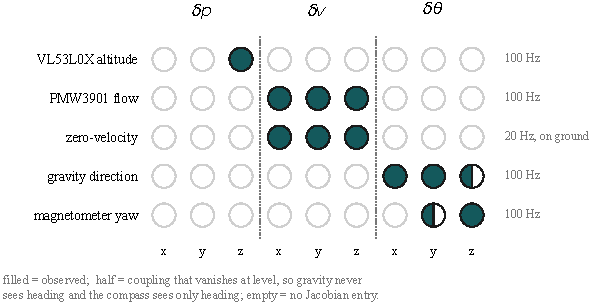
\includegraphics[width=\columnwidth]{fig_estimator.pdf}
\caption{Measurement Jacobian structure. Every update is a sequence of scalar
updates with an individual innovation gate, which makes each axis
independently rejectable and avoids a matrix inversion on the target. Note
that horizontal position is never measured by anything.}
\label{fig:estimator}
\end{figure}

\subsection{Formulation}

The estimator is a nine-error-state Kalman filter. The nominal state carries
navigation-frame position and velocity and a body-to-navigation quaternion;
the filter's state is the error in that nominal state:
\begin{equation}
\delta\mathbf{x} =
\begin{bmatrix} \delta\mathbf{p}_N & \delta\mathbf{v}_N & \delta\boldsymbol{\theta}_B \end{bmatrix}^{\!\top}
\in \mathbb{R}^{9}.
\end{equation}
Attitude error is a right-multiplicative body-frame rotation vector,
$R_{\text{true}} \approx R_{\text{nom}}\exp([\delta\boldsymbol{\theta}_B]_\times)$,
so the filter carries no quaternion norm constraint, has no singularity, and
its small-angle linearisation is always valid because the error is reset to
zero after every injection~\cite{sola2017}.

Prediction runs every control cycle. The gyro increment rotates the quaternion
by right multiplication to match the error convention; specific force is
rotated to navigation, gravity is removed, and translation integrates forward.
The discrete error transition is first order, $A \approx I + F\,\Delta t$, with
three non-trivial blocks:
\begin{equation}
\frac{\partial \delta\mathbf{p}}{\partial \delta\mathbf{v}} = I\,\Delta t,
\quad
\frac{\partial \delta\mathbf{v}}{\partial \delta\boldsymbol{\theta}} = -R[\mathbf{a}_B]_\times \Delta t,
\quad
\frac{\partial \delta\boldsymbol{\theta}}{\partial \delta\boldsymbol{\theta}} = I - [\boldsymbol{\omega}_B]_\times \Delta t.
\end{equation}

\subsection{Measurements}

Fig.~\ref{fig:estimator} shows which error states each measurement can reach.
Three design decisions are worth stating.

\emph{Optical flow uses a translation-only update.} A body-velocity update
with an attitude Jacobian exists in the estimator but is not called. The
update actually used observes velocity through $\mathbf{v}_B = R^\top
\mathbf{v}_N$ but deliberately omits the attitude partial, so an unverified
flow axis, sign or scale can never rotate the quaternion. Both scalar axes
must pass their gates for the sample to count, so a failed axis cannot hide
behind a healthy one.

\emph{Gravity aiding is decimated 4:1} to 100~Hz, with the standard deviation
scaled by $1/\sqrt{4}$ so that one update in four delivers the same correction
per unit time. The full three-axis update with its covariance propagation was
approximately half the estimator cost, and the gyro already carries everything
above a few hertz.

\emph{Gravity and the magnetometer are structurally separated.} The gravity
update's Jacobian is built from the skew of navigation~$+Z$ expressed in body,
which at level reduces to $\delta\theta_x$ and $\delta\theta_y$ only; it can
never observe heading. The magnetometer Jacobian is
$[\,0\;\ldots\;\sin\theta/\cos\phi\;\;\cos\theta/\cos\phi\,]$, which at level
reduces to $\delta\theta_z$ alone.

\subsection{Cross-check against a complementary filter}

An independent complementary filter with a 0.133~s time constant runs on the
same samples. Each cycle the two attitude solutions are compared, and the
filter output is used only if they agree within tolerance and both angles are
under $80^{\circ}$; otherwise the complementary estimate is used and a flag is
raised. This is a runtime guard against estimator divergence rather than a
fallback of last resort, and it costs almost nothing.

%% ===========================================================================
\section{Control Architecture}
\label{sec:control}

\begin{figure*}[!t]
\centering
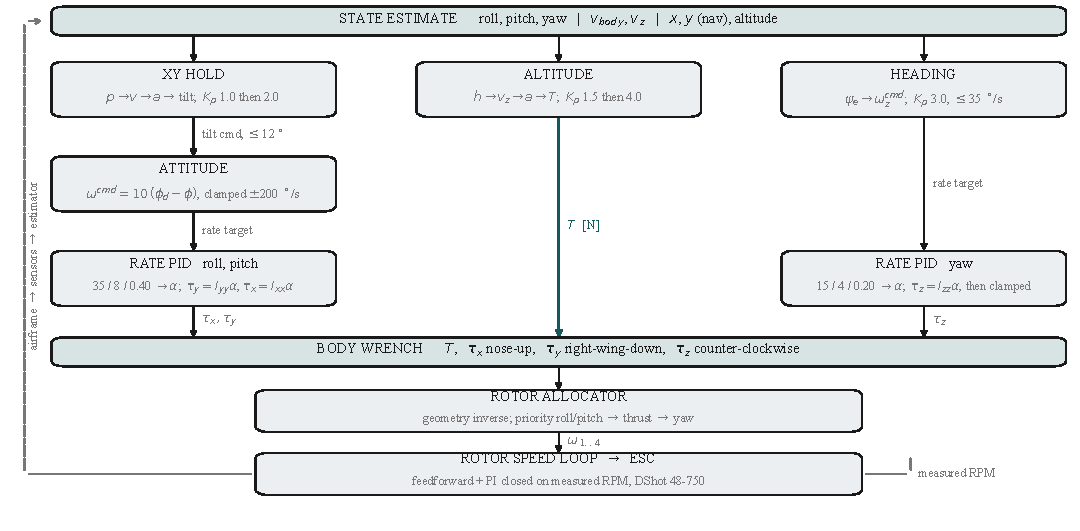
\includegraphics[width=\textwidth]{fig_cascade.pdf}
\caption{Control cascade. All blocks execute at 400~Hz within one control
step. The three outer loops are parallel and independent; altitude bypasses
the attitude and rate loops entirely and writes directly into the wrench,
which is what allows the allocator to protect it from the torque axes. The
only closed measurement loop below the wrench is rotor speed.}
\label{fig:cascade}
\end{figure*}

Fig.~\ref{fig:cascade} shows the complete cascade and Table~\ref{tab:gains}
lists the gains and limits. The loops are separated in bandwidth by roughly a
factor of three per stage.

\begin{table}[!t]
\caption{Control Gains and Limits}
\label{tab:gains}
\centering
\footnotesize
\begin{tabular}{@{}llrr@{}}
\toprule
Loop & Input $\rightarrow$ output & Gain & Limit \\
\midrule
Position   & position err $\rightarrow$ velocity    & 1.00 & 0.50 m/s \\
Velocity   & velocity err $\rightarrow$ tilt        & 2.00 & 1.50 m/s$^2$ \\
Attitude   & tilt err $\rightarrow$ body rate       & 10.0 & 200 \dps \\
Rate r/p   & rate err $\rightarrow$ $\alpha$        & 35 / 8 / 0.40 & 60 rad/s$^2$ \\
Altitude   & altitude err $\rightarrow$ $v_z$       & 1.50 & 0.50 m/s \\
Vert.\ vel & $v_z$ err $\rightarrow$ thrust         & 4.00 & 3.00 m/s$^2$ \\
Heading    & heading err $\rightarrow$ yaw rate     & 3.00 & 35 \dps \\
Rate yaw   & rate err $\rightarrow$ $\alpha$        & 15 / 4 / 0.20 & authority \\
Rotor      & $\omega$ err $\rightarrow$ DShot       & 0.15 / 2.0 & 48--750 \\
\bottomrule
\end{tabular}
\end{table}

\subsection{Rate loops}

One PID implementation serves all three axes. It returns an angular
acceleration, and the caller multiplies by the axis inertia:
\begin{equation}
\alpha_{\text{cmd}} = k_p e + k_i\!\!\int\!\! e\,dt + k_d \dot{e}_f,
\qquad
\tau = I_{\text{axis}}\,\alpha_{\text{cmd}}.
\end{equation}
The integral clamp bounds the \emph{contribution} rather than the accumulator:
$\pm 60/k_i$ means the integral term can never exceed 60~rad/s$^{2}$ whatever
$k_i$ is set to. For roll that is 0.060~N$\cdot$m out of 0.339~N$\cdot$m
available, or 18\%. For yaw the same bound corresponds to 0.122~N$\cdot$m
against 0.042~N$\cdot$m available---nearly three times the airframe's total
yaw authority---which is why yaw alone carries the conditional integration
described below.

Roll is a rotation about $+Y$ and pitch about $+X$, so the roll loop closes on
$\omega_y$ and produces $\tau_y$, and the pitch loop closes on $\omega_x$ and
produces $\tau_x$. Keeping that pairing explicit in the variable names is the
principal defence against the class of fault described in the introduction.

\subsection{Attitude}

A single proportional gain, deliberately without integral or derivative
action, mapping tilt error to a rate target for the inner loop. The cascade
requires the rate loop to remain roughly $3.5\times$ faster than the attitude
loop; raising the attitude gain alone purchases overshoot rather than
authority.

\subsection{Altitude}

Two proportional stages produce a thrust command:
\begin{equation}
T = \frac{m\left(g + a_z\right)}{\cos\phi\,\cos\theta},
\qquad
a_z = k_{v_z}\!\left(v_z^{\text{cmd}} - v_z\right),
\end{equation}
with the tilt cosine floored at 0.5 and the result clamped to
$[0.35, 1.90]\,W$. Division by the tilt cosine prevents banking from sagging
the altitude.

There is no integral term anywhere in the vertical cascade. This is a design
choice with a direct consequence: no modelling error can be absorbed, so any
error in mass or in $\kF$ appears as a permanent altitude offset.
Section~\ref{sec:results} quantifies exactly that.

\subsection{Horizontal position}

Two proportional stages again. When held, position error is formed in the
navigation frame and the resulting velocity target is rotated into the body
frame before comparison against the measured body velocity, so the heading
appears once in the feed-forward path rather than inside the feedback loop.
The commanded acceleration becomes a tilt through
$\phi_d = \mathrm{atan2}(a_x, g)$ and
$\theta_d = \mathrm{atan2}(-a_y, g)$; the negation on pitch is physically
required, since a right-handed nose-up pitch accelerates the aircraft
backwards.

Position hold is gated on flow health, both flow axes accepted, estimator
health, confirmed airborne state, height above 0.30~m, vertical speed below
0.20~m/s, tilt below $6^{\circ}$, yaw rate below 25~\dps, and---the condition
absent from the previous build---evidence within the current flight that the
yaw loop is behaving: yaw rate within 10~\dps\ and heading error within
$8^{\circ}$, continuously for three seconds while airborne. Disarming clears
the proof, so every flight re-earns it.

Because nothing measures horizontal position, the navigation-frame coordinates
are integrated flow velocity and they drift. The captured target lives in the
same drifting frame, so slow common-mode drift cancels; the hold is
station-keeping against a velocity reference, not position hold in any
absolute sense.

\subsection{Heading}

Yaw stabilisation is never released. Unlike the other axes, where an engaged
stick surrenders the axis without resistance, the yaw stick commands a rate
through the same loop that holds heading, and the heading target is
re-captured once the axis settles below 8~\dps\ for 300~ms.

The rate PID output is then clamped to what the rotors can actually deliver at
the collective already committed to thrust:
\begin{equation}
\left|\tau_z\right|_{\max} = 4\,\kM \min\!\left(c - u_{\min},\; u_{\max} - c\right),
\qquad c = \frac{T}{4\kF}.
\label{eq:yawauth}
\end{equation}
Critically, when the clamp acts, exactly the discarded amount is removed from
the integrator:
\begin{equation}
\int e\,dt \;\mathrel{-}=\; \frac{\tau_z - \tau_z^{\text{clamped}}}{I_{zz}\,k_i}.
\end{equation}
Clamping alone would be insufficient. The integrator would still charge
against a saturated actuator and, once charged, could not discharge. An
unachievable setpoint is an open loop with extra steps.

%% ===========================================================================
\section{Control Allocation}
\label{sec:alloc}

\begin{figure}[!t]
\centering
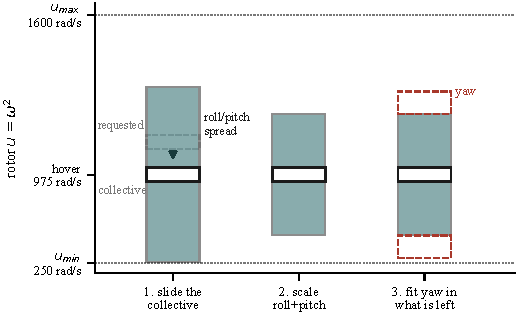
\includegraphics[width=\columnwidth]{fig_alloc.pdf}
\caption{Rotor-speed budget spent in priority order. Under the earlier policy
the collective sled to accommodate \emph{yaw} and all three torque axes were
scaled by one common factor; a single yaw demand four times the achievable
value therefore dumped thrust and stripped roll and pitch of authority at the
moment the aircraft was tilting.}
\label{fig:alloc}
\end{figure}

Because \eqref{eq:fwdT}--\eqref{eq:fwdZ} are linear in $u_i$, the inverse is
closed form:
\begin{equation}
\begin{aligned}
u_1 &= c_T + c_X + c_Y - c_Z, &\quad u_2 &= c_T + c_X - c_Y + c_Z, \\
u_3 &= c_T - c_X - c_Y - c_Z, &\quad u_4 &= c_T - c_X + c_Y + c_Z,
\end{aligned}
\end{equation}
with $c_T = T/4\kF$, $c_X = \tau_x/4\kF a_y$, $c_Y = \tau_y/4\kF a_x$ and
$c_Z = \tau_z/4\kM$. Rotor speeds are bounded to $[250, 1600]$~rad/s; the
non-zero floor exists because allowing a rotor to stop in flight costs
hundreds of milliseconds to recover and is a common way to lose an axis.

The demand frequently does not fit, and what happens then is a priority
decision that follows from the authority asymmetry rather than from taste
(Fig.~\ref{fig:alloc}):

\begin{enumerate}
\item \textbf{Slide the collective} so that the roll/pitch differential fits.
Yaw is excluded from this calculation.
\item \textbf{Scale roll and pitch together} by one common factor if they
still do not fit. One factor, so that the commanded tilt \emph{direction}
survives---independently clipping the two rotates the torque vector and is a
classic cause of coupled wobble near full deflection.
\item \textbf{Fit yaw into whatever range remains}, scaling it down, to zero
if necessary. Nothing above moves to accommodate it.
\end{enumerate}

The argument for scaling roll and pitch jointly never applied to yaw, which is
a physically separate actuation mechanism rather than another component of the
same thrust-difference vector. The allocator reports the wrench it actually
achieved rather than the one requested, which is what the parameter identifier
of Section~\ref{sec:km} consumes, and it exposes all three clip conditions in
telemetry.

%% ===========================================================================
\section{Rotor Speed Loop}
\label{sec:rotor}

Four independent controllers close on measured mechanical rotor speed:
\begin{equation}
d_i = \hat{g}_i\,\omega_i^{\text{sp}} + k_p e_i + k_i\!\!\int\!\! e_i\,dt,
\end{equation}
where $\hat{g}_i$ is a slowly learned DShot-per-rad/s gain. The relation is
not through the origin---ESCs have an idle offset and the curve bends---so the
loop models gain only and lets the integrator absorb the offset.

This layer is what makes the rigid-body model above meaningful. With an
open-loop mixer, every motor nonlinearity, every battery sag and every
propeller difference appears directly as an attitude disturbance for the outer
loop to chase. Closing the rotor loop turns the four actuators into something
that approximates the linear map the allocator inverted.

Four protections are worth recording, each traceable to an observed failure:

\emph{Setpoint slew limiting} at 4000~rad/s$^{2}$. A bench step from standstill
to 500~rad/s overshot to 635~rad/s because the integrator accumulated during
the $\approx$50~ms the motor physically required. Harmless with propellers
removed; at hover it would be a transient 60\% thrust excursion, since thrust
goes as $\omega^{2}$.

\emph{Conditional integration} inside a band of
$\max(60,\,0.10\,\omega^{\text{sp}})$~rad/s. A flat 60~rad/s band deadlocked
the loop in flight: an 81~rad/s standing offset lay outside the band, so the
integrator froze, leaving only $k_p e \approx 12$ DShot counts against the 90
required, which held the error at 81.

\emph{Telemetry-gap handling.} When a rotor's speed measurement goes stale the
loop holds its integrator, stops learning and runs feedforward against an
open-loop first-order motor estimate, rather than integrating against a frozen
measurement and slamming the motor when telemetry returns.

\emph{Anti-windup} that unwinds exactly the excess when the command is pinned
at either rail.

Ground idle is driven through this same loop at 500~rad/s rather than by a
fixed DShot value, so the slewed setpoint, the learned gain and the integrator
are all converged and continuous at the moment the climb state takes over. The
previous fixed-value idle bypassed the loop, and the first climb cycle
therefore began its slew from zero and commanded minimum throttle---a full
thrust cut at the instant of takeoff.

%% ===========================================================================
\section{Implementation}
\label{sec:impl}

The firmware is approximately 12{,}300 lines of C++ compiled with
\texttt{arduino-cli} against the \texttt{esp32:esp32} core, occupying 77\% of
flash and 15\% of RAM.

\subsection{Task structure and timing}

The control step runs at 400~Hz (2500~\textmu s) from the main loop. Serial
command handling and the three polled sensors are serviced on every pass
rather than only when the control step finishes early, because coupling
command responsiveness to control-step duration made the console arbitrarily
laggy with no indication why. The optical-flow sensor runs in a dedicated
FreeRTOS task pinned to the opposite core and delivers samples through a
queue, since its burst read is long enough to disturb the control cadence.

Timing is instrumented and published: mean and worst-case control-step
duration, and the number of main-loop passes per control step, which is the
headroom figure---a value of one means nothing else can run.

\subsection{Failsafe and arming}

Signal loss is declared at 300~ms. The age comparison is signed:
{\footnotesize
\begin{verbatim}
int32_t age = (int32_t)(now - lastPkt);
lost = (lastPkt == 0) || (age > 300);
\end{verbatim}
}
This was an unsigned subtraction and was the cause of repeated unexplained
disarms. The current time is sampled once at the top of the control cycle,
but the ESP-NOW receive interrupt can fire afterwards and store a later
timestamp; the unsigned difference then wrapped to approximately
$4.29\times10^{9}$, trivially exceeding the timeout. The log recorded ``last
packet 4294967295~ms ago'' on a run whose worst genuine gap was 52~ms.

Disarm causes are evaluated in a fixed order with signal loss tested first,
because the failsafe path zeroes the arm flag before the check runs; testing
the arm flag first reported every link dropout as an operator disarm.

Arming requires the throttle stick near centre, since throttle is a centred
axis in this design---centre holds altitude, up climbs, down descends---and a
refusal is logged with the actual stick value.

\subsection{Flight states and engagement logic}

\begin{figure*}[!t]
\centering
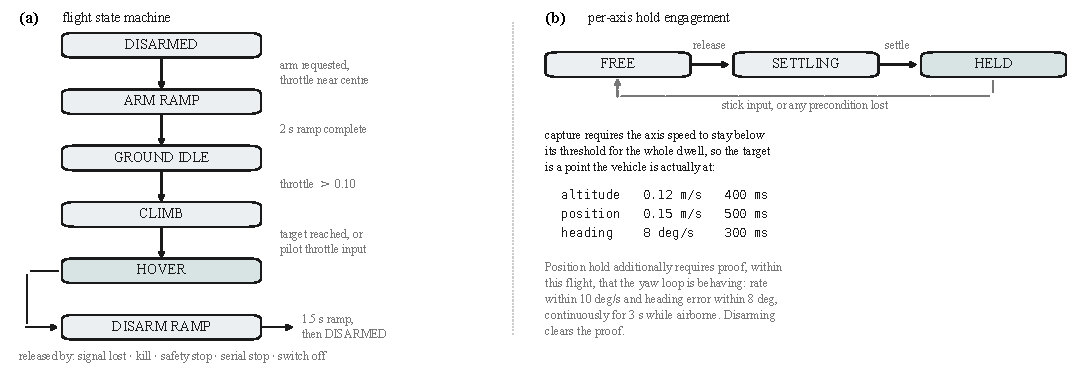
\includegraphics[width=\textwidth]{fig_states.pdf}
\caption{(a) Flight state machine. Arming spins the rotors to idle and stops;
the aircraft stays on the ground until the throttle stick is first raised.
(b) The settle-then-capture logic shared by all three holds. The cost is a
small drift during the settle; the benefit is that every captured target is a
point the vehicle is actually at and nearly stationary over.}
\label{fig:states}
\end{figure*}

Fig.~\ref{fig:states}(a) shows the flight state machine. Arming ramps the
rotors to idle over two seconds and stops there; the aircraft remains on the
ground until the throttle stick is first raised, then climbs to the hover
setpoint under closed-loop vertical velocity control and holds hands-off.
Ground idle is commanded through the rotor speed loop rather than as a fixed
actuator value, for the handoff reason given in Section~\ref{sec:rotor}.

Three holds share one settle-then-capture state machine,
Fig.~\ref{fig:states}(b). While a stick is held the axis is free. On release
the axis does not capture immediately, because the vehicle still carries
momentum and would latch a point it is moving away from; instead it waits for
the measured speed on that axis to remain below a threshold for a dwell, then
captures.

A separate one-way latch distinguishes ``the state machine is in a flying
state'' from ``the aircraft is off the ground''. The latter requires
$\geq0.15$~m for 300~ms continuously and, once set, is not cleared by a brief
dip toward the floor. Conflating the two previously allowed a hold to capture
a 0.25~m target while the rangefinder read 0.03~m and the aircraft sat on the
bench. A related interaction is that altitude hold is inhibited entirely
during the climb state: permitting it earlier let the hold capture a target
just above the airborne threshold, which then satisfied the climb-complete
test and truncated every takeoff at roughly 0.20~m.

%% ===========================================================================
\section{Testing and Results}
\label{sec:results}

\subsection{Method}

Results below are drawn from telemetry captured over the serial link at 5~Hz
during a hover flight on 15 August 2026, logged as 5694 telemetry frames of
which 917 were in a flying state and 898 in hover. Analysis used the longest
contiguous airborne segment, 348 samples spanning 69~s, so that the
reconstructed time axis never spans a disarm. Steady-hover statistics use the
603 frames with $|v_z| \leq 0.05$~m/s and altitude hold engaged.

\stub{No instrumented bench test rig exists. Rate-loop step responses, closed
loop bandwidth and phase margin have not been measured; the gains in
Table~\ref{tab:gains} were reached by flight observation. A single-axis pivot
rig with the aircraft constrained to one degree of freedom, driven by the
\texttt{ratelog} serial stream, would give measured step responses per axis.
Report rise time, overshoot and settling time for each of roll, pitch and yaw.}

\subsection{Attitude regulation}

\begin{figure*}[!t]
\centering
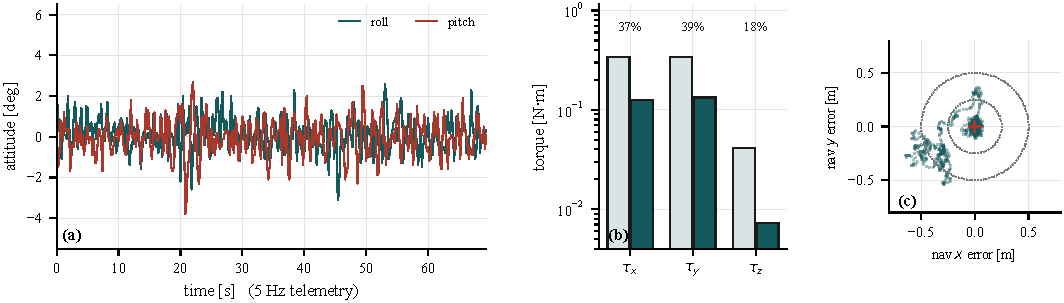
\includegraphics[width=\textwidth]{fig_results.pdf}
\caption{(a) Attitude over the 69~s hover segment, hands off.
(b) Peak commanded torque against available authority, logarithmic scale;
percentages are utilisation. (c) Horizontal position error while the hold was
engaged, with 0.25 and 0.50~m reference circles.}
\label{fig:results}
\end{figure*}

Fig.~\ref{fig:results}(a) shows attitude across the hover segment with no
pilot input. Roll held a standard deviation of $1.09^{\circ}$ and pitch
$1.17^{\circ}$, with 95th-percentile absolute excursions of $2.00^{\circ}$ and
$2.20^{\circ}$. Mean attitude was within $0.2^{\circ}$ of level on both axes,
indicating that the boot-time attitude reference happened to be close to true
level on this flight.

Fig.~\ref{fig:results}(b) shows torque utilisation. Peak commanded torque
reached 37\% of available authority in pitch, 39\% in roll and 18\% in yaw.
The margin in roll and pitch is deliberate; the margin in yaw exists because
the demand clamp of \eqref{eq:yawauth} is doing its job.

Across all 917 airborne frames the allocator reported \emph{no} saturation of
any kind---no clipped yaw demand, no clipped yaw allocation, no scaled
roll/pitch. On the preceding build, the equivalent flight ended in an
excessive-tilt abort at $39.9^{\circ}$ of roll with two rotors pinned at the
upper rail and two at the lower.

\subsection{Altitude and the thrust model}

\begin{figure}[!t]
\centering
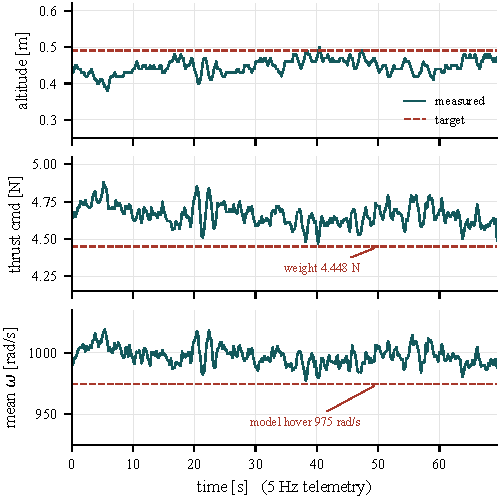
\includegraphics[width=\columnwidth]{fig_hover.pdf}
\caption{Hover segment. The altitude hold captured at 0.50~m and held to
22~mm standard deviation, but settled 55~mm below target. The commanded
thrust and the measured rotor speed together identify the cause.}
\label{fig:hover}
\end{figure}

Altitude hold captured close to the 0.50~m hover setpoint and held with a
standard deviation of 22~mm, but settled at a mean of 0.442~m---a persistent
offset of $-55$~mm against the captured target
(Fig.~\ref{fig:hover}). The vertical loop is not misbehaving. Propagating the
measured mean altitude error and vertical velocity through the two
proportional stages predicts a thrust command of 4.656~N; the logged mean was
4.662~N, an agreement of 0.1\%. The loop is doing exactly what it is told.

The offset is an equilibrium, and it exists because the vertical cascade
contains no integral term. Its magnitude identifies the residual model error.
The aircraft hovered at a mean rotor speed of 998~rad/s against a modelled
hover speed of 975~rad/s. Inverting \eqref{eq:fwdT} at the measured speed
gives an implied $\kF$ of $1.117\times10^{-6}$ against the modelled
$1.170\times10^{-6}$: the model over-predicts thrust by 4.8\%, corresponding
to $C_T \approx 0.138$ rather than the compiled 0.145.

This is the third successive correction in the same direction, and the reason
is instructive. Each identification was performed at a higher hover altitude
than the last, and each found the previous value optimistic, because ground
effect makes a given rotor speed produce more thrust than in free air. An
earlier attempt to explain the same offset by raising the modelled \emph{mass}
was withdrawn: the supporting check compared commanded against delivered
thrust, but the allocator obtains rotor speed by dividing commanded thrust by
the model $\kF$ and delivered thrust is recovered by multiplying by the same
model $\kF$, so those two figures agree by construction whenever the rotor
loop tracks, regardless of how wrong $\kF$ is. The diagnostic signature was
that the implied mass followed each edit rather than remaining constant.

\subsection{Position and heading hold}

Heading hold was engaged for 84\% of airborne frames and held a mean absolute
error of $1.20^{\circ}$ with a worst case of $13.5^{\circ}$.

Position hold engaged for 74\% of airborne frames, after satisfying the
yaw-stability proof. Performance varied substantially between flights. On the
flight analysed here the radial error averaged 0.242~m with a worst case of
0.704~m over 682 held frames (Fig.~\ref{fig:results}(c)); on a shorter hold
earlier the same afternoon it averaged 0.042~m with a worst case of 0.103~m
over 162 frames. The scatter shows a tight cluster near the target with one
sustained excursion, consistent with accumulated drift in the unobservable
horizontal position states rather than with loop instability.

\stub{The position-hold variation between flights is unexplained. Candidate
causes are floor texture (flow surface quality averaged 79 on the worse flight
against 98--122 on the better ones), height above the floor, and ambient
light. A controlled comparison over three surfaces at a fixed height, logging
flow surface quality alongside radial error, would separate them.}

\subsection{Computational load}

Mean control-step duration was 1276~\textmu s against the 2500~\textmu s
budget, with a worst case of 2025~\textmu s. The main loop completed at least
133 passes per control step, so the asynchronous sensors and the serial
console were never starved. Optical flow was healthy on 99\% of frames.

\subsection{Summary}

\begin{table}[!t]
\caption{Hover Flight Results, 15 August 2026}
\label{tab:results}
\centering
\footnotesize
\begin{tabular}{@{}llr@{}}
\toprule
Quantity & Condition & Value \\
\midrule
Roll dispersion        & 917 airborne frames & $1.09^{\circ}$ sd \\
Pitch dispersion       & 917 airborne frames & $1.17^{\circ}$ sd \\
Altitude dispersion    & 603 steady frames   & 22 mm sd \\
Altitude offset        & vs captured target  & $-55$ mm \\
Heading error          & 755 held frames     & $1.20^{\circ}$ mean \\
Radial position error  & 682 held frames     & 0.242 m mean \\
Allocator saturation   & 917 airborne frames & 0 frames \\
Peak torque, roll      & fraction of authority & 39\% \\
Peak torque, yaw       & fraction of authority & 18\% \\
Control step, mean     & 2500 \textmu s budget & 1276 \textmu s \\
Control step, worst    & 2500 \textmu s budget & 2025 \textmu s \\
\bottomrule
\end{tabular}
\end{table}

Table~\ref{tab:results} collects the results. The controller achieves stable
hands-off hover with substantial authority margin on every axis and no
allocator saturation, which was the primary objective. The residual defects
are a quantified thrust-model error and an unvalidated horizontal position
hold.

%% ===========================================================================
\section{In-Flight Parameter Identification}
\label{sec:km}

The rotor drag coefficient is the one physical parameter never characterised
for this airframe. An in-flight identifier estimates it from the yaw dynamics:
\begin{equation}
\underbrace{I_{zz}\dot{\omega}_z + \dot{H}_z}_{y}
 = -\kM D - c\,\omega_z,
\qquad
D = u_1 - u_2 + u_3 - u_4,
\end{equation}
where $H_z$ is net rotor angular momentum about $+Z$ and $c$ is an
aerodynamic yaw damping term estimated jointly. The damping term was added
after early attempts failed: in a sustained turn both $\dot{\omega}_z$ and
$\dot{H}_z$ approach zero while $D \neq 0$, so the only available fit is
$\kM \rightarrow 0$.

Estimation is normalised least-mean-squares, gated on an explicit
commissioning flag, confirmed airborne state, fresh telemetry on all four
rotors, sufficient excitation, an unsaturated allocator and near-level
attitude, and hard-clamped to a physical band.

\stub{Identification has not succeeded. Three attempts were run and all three
were rejected. The controller still uses the seed value, $\kM = 1.17\times
10^{-8}$. The obstacle is that $\kM$ and $c$ are collinear under the flight
conditions achieved so far: with slow yaw close to the ground, $D$ and
$\omega_z$ move together and the regression cannot separate rotor drag from
airframe damping. Removing the magnetometer from the loop did not change the
outcome, which eliminates compass coupling as the cause. What is required is a
flight condition with yaw excitation that is not correlated with rotor
differential---a deliberate swept-frequency yaw input at a hover height clear
of ground effect. Report the converged $\kM$, the spread fraction, and the
damping coefficient $c$; a plausible $c$ is of order 0.009~N$\cdot$m per
rad/s.}

%% ===========================================================================
\section{Limitations}
\label{sec:limits}

Several known defects are recorded here rather than omitted.

\emph{Magnetometer coupling.} The QMC5883P shifts by several degrees with
motor current owing to its proximity to the power leads. Heading hold is
consequently flown with its proportional gain set to zero, which leaves the
compass fusing into the estimator but removes its authority over the motors.
The results in Section~\ref{sec:results} were obtained in that configuration.
Relocating the sensor is a prerequisite for closing the heading loop.

\emph{Attitude reference.} As described in Section~\ref{sec:sensors}, the
level reference is whatever pose the aircraft occupied at power-up.

\emph{Horizontal position is unobservable.} No sensor measures it, so it is
integrated flow velocity and drifts without bound.

\emph{Rotor feedforward seed.} The rotor loop seeds its feedforward gain as a
fixed DShot value divided by the modelled hover speed. Because the hover speed
is derived from $C_T$, correcting the thrust model silently moved the seed;
at the present $C_T$ it is approximately 10\% low. The learned gain and the
integrator converge it out within a few hundred milliseconds, but the coupling
is unintended.

\emph{Flow de-rotation gains} were carried over from an earlier empirical fit
and re-expressed in the right-handed frame. They are algebraically identical
to what was previously applied, but the original fit absorbed scale error and
was never independently validated.

%% ===========================================================================
\section{Conclusion}

A model-based flight controller for a 163~mm quadrotor was implemented on a
single ESP32, using a nine-error-state Kalman filter for estimation, a
six-deep cascade expressed entirely in physical units, a control allocator
derived from rotor geometry, and an innermost loop closed on rotor speed
recovered from bidirectional DShot telemetry.

Two design decisions proved decisive in flight. Deriving the allocation matrix
from geometry rather than writing it down eliminated the class of sign fault
that had defeated the previous build, and the same discipline applied to
sensor mounting transforms let the corrected yaw convention be introduced
without disturbing the roll and pitch behaviour that already worked. Ordering
the saturation policy by physical authority---roll and pitch first, then
thrust, then yaw---removed the coupling by which an impossible yaw demand
could previously dump collective thrust and strip the attitude loops of
control at the moment they were most needed; the flight reported here recorded
no allocator saturation of any kind across 917 frames.

Expressing gains in physical units also made the remaining error diagnosable
rather than merely visible. A persistent 55~mm altitude offset was shown to be
an exact equilibrium of a cascade with no integral term, and its magnitude
identified a 4.8\% error in the modelled thrust coefficient. That is a
correction to a physical constant, not a gain to be retuned.

Remaining work is the relocation of the magnetometer, identification of the
rotor drag coefficient under an uncorrelated yaw excitation, a bifilar
measurement of the inertia tensor, and instrumented rate-loop step responses.

%% ===========================================================================
\section*{Acknowledgment}

\stub{Acknowledgements, advisor and any course or laboratory support.}

\balance
\bibliographystyle{IEEEtran}
\bibliography{refs}

\end{document}
